\documentclass[12pt]{article}

\usepackage{amsmath}
\usepackage{amssymb}
\usepackage{amsthm}
\usepackage{graphicx}
\usepackage{float}

\title{Demystifying the Projection Matrix in 3D Graphics Transformations}
\author{Spencer T. Parkin}

\begin{document}
\maketitle

Of all the standard matrices for 3D computer graphics, the projection matrix stands out as the most intimidating and least understood.  Like most matrices, however, once you get to know them, they're really not all that bad.

Enter camera space.  This is the space where all 3D objects ultimately land to be viewed before going to projection space where they can be rasterized to the screen.  The projection matrix is simply what takes vertices from camera space to projection space.  So before we can begin to contemplate such a matrix, we need to clearly define each of these two spaces.

\section*{Camera Space}

Different graphics systems have their different conventions, but typically, camera space is where we imagine the camera as an eye-point at the origin of the 3D cartesient coordinate system, stairing down the -Z axis, with the +X axis to the right, and the +Y axis pointing upward.  An object is transformed from its object space to world space, and then world space to where it can be seen (or not seen) by the camera in the camera space thus described.

But we have to be more specific.  For example, what is the field of vision for the camera?  And what are the extents to which the camera can see?  This is where the frustum comes into play.  The frustum is simply a pyramid with the top chopped off.  Where the pointy part of the pyrmaid would have been, we have the eye point of the camera.  The center of the base of the pyramid is exactly where the camera is looking.  The 6 sides of this chopped-off pyrmaid form the frustum, or viewing extents of the camera.  The inside of the frustum is the relavant camera space.  Whatever falls into this space, barring any possible occlusion by other objects, is visible, and is what we want to map into projection space.

\section*{Projection Space}

This space models the place where clipping and rasterization can be performed, or at least imagined.  Again, you're at the origin, and you're looking down the $-Z$ axis.  The $+X$ axis is to the right, and the $+Y$ axis is upward.  So what's the difference?  Instead of a frustum bounding the relevant viewing area, we have a box with edges meeting at right angles, usually of 2 units width and height, and just 1 unit of depth, centered at the origin with respect to the $XY$-plane, width all depth in the range $[0,-1]$.  These dimensions make it natural and easy to map the space to an on or off-screen image, clip primitives against its extents, and also to perform depth testing.

\section*{The Projective Effect}

With our spaces defined, it is now easy to imagine a mapping from camera space to projection space that produces the projective effect; that is, the effect where things closer to the eye appear larger than if they were located further away.  The morphing, if you will, of the frustum to the projection box will cause objects in camera space to distort as they travel to projection space.  For example, a road which, geometrically, has a consistent width in camera space, will appear to narrow into the distance in projection space.

\section*{The Projective Mapping}

We can now begin to rigously define our mapping from camera space to projection space.  We'll start with a 2D example before generalizing to 3D space.  Consider the following two equations.
\begin{equation*}
q_x = \frac{p_x}{p_y\tan\frac{\theta}{2}}
\end{equation*}
\begin{equation*}
q_y = \frac{p_y-n}{f-n}
\end{equation*}
Here, $P=(p_y,p_x)$ is a point in camera space, and $Q=(q_x,q_y)$, is $P$ projected into projection space.
The angle $\theta$ is the viewing angle, $n$ is our distance along the $+Y$ axis to the near clipping plane of the frustum, and $f$ is the distance to the far clipping plane.  With a little trigonometry, and the aide of figures \ref{fig1} and \ref{fig2}, it's not hard to see why these equations make sense.
\begin{figure}
\centering
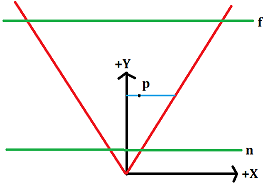
\includegraphics{fig1}
\caption{A point $p$ in camera space with the near and far planes (green) and the left and right sides of the viewing extent (red), meeting at an angle $\theta$.}
\label{fig1}
\end{figure}
\begin{figure}
\centering
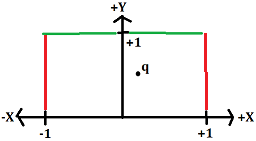
\includegraphics{fig2}
\caption{A point $q$, the projection of $p$ from camera space into projection space; the space having width in the range $[-1,1]$, and depth in the range $[0,1]$.}
\label{fig2}
\end{figure}
One will see right away, however, that these are not linear transformations.  Consequently, we can't encode this type of transformation in a $2\times 2$ matrix.  Further, we'll find that the equation for $q_y$, although ideal, will have to be substituded with an alternative way of mapping the point $P$'s depth along the $Y$ axis in the range $[n,f]$ to $[0,1]$.

The answer, then, (as discovered by August Ferdinand Mobius), is to work in higher dimensions in conjunction with the notion of homogenous coordinates.  In this system, a point $P$ is extended to 3D space as the point $P=(p_x,p_y,1)$, and we say that any point $R=(r_x,r_y,r_z)$ is equivilent to $P$ if and only if $r_x/r_z=p_x$ and $r_y/r_z=p_y$.  This creates an equivilance relation in 3D space, and we say that $P$ is the homogenized form of $R$.

With this trick up our sleaves, we can now try to formulate equations similar to those above, as follows, in matrix form.

\begin{equation*}
\left[
\begin{array}{ccc}
\frac{1}{\tan(\theta/2)} & 0 & 0 \\
0 & a & b \\
0 & 1 & 0 \\
\end{array}
\right]\left[
\begin{array}{c}
p_x \\
p_y \\
1
\end{array}
\right] = \left[
\begin{array}{c}
\frac{p_x}{\tan(\theta/2)} \\
ap_y + b \\
p_y
\end{array}
\right] \sim \left[
\begin{array}{c}
q_x \\
a + \frac{b}{p_y} \\
1
\end{array}
\right]
\end{equation*}
Here, I've filled in the $3\times 3$ matrix with everything we know needs to be there to achieve our ends, while leaving unknown values of the matrix parameterized; in this case, with the variables $a$ and $b$.  What we're now looking for is a mapping from the range $n\leq p_y\leq f$ to the following.
\begin{equation*}
0\leq a + \frac{b}{p_y}\leq 1.
\end{equation*}
One way to go about this is to setup equations for the top and bottom of these ranges, solve the resulting system, and then hope the inequalities continue to hold.  Doing so, our system becomes as follows.
\begin{equation*}
0 = a + \frac{b}{n}
\end{equation*}
\begin{equation*}
1 = a + \frac{b}{f}
\end{equation*}
Solving this system for $a$ and $b$, we're able to complete our earlier $3\times 3$ matrix as follows.
\begin{equation*}
\left[
\begin{array}{ccc}
\frac{1}{\tan\theta/2} & 0 & 0 \\
0 & \frac{f}{f-n} & \frac{-fn}{f-n} \\
0 & 1 & 0
\end{array}
\right]
\end{equation*}
And there we have it!  This is our projection matrix.  The reader can check that the inequalities still hold, but will also notice that our mapping into the depths of projection space is not linear, but curved in a way that can be problamatic when testing Z-values close to the far clipping plane due to loss of precision.  Nevertheless, it works well enough.

\section*{Generalizing to 3D}

Naturally, to extend what we have to 3D space, we'll need a $4\times 4$ matrix, and work with homogenized coordinates in 4D space.  The generalization is easy.  Just consider the following matrix product.

\begin{equation*}
\left[
\begin{array}{cccc}
\frac{1}{\tan\theta/2} & 0 & 0 & 0 \\
0 & \frac{1}{\tan\phi/2} & 0 & 0 \\
0 & 0 & \frac{-f}{f-n} & \frac{fn}{f-n} \\
0 & 0 & 1 & 0
\end{array}
\right]\left[
\begin{array}{c}
p_x \\
p_y \\
p_z \\
1
\end{array}
\right]
\end{equation*}

Here we can see that $\theta$ is our horizontal field of vision, while $\phi$ is the vertical field of vision.  Aside from being of higher dimension, you'll also notice that the signs of the entries involving the near and far clipping distance have flipped from our earlier version.  It's not hard to see why if you go through the derivision again as earlier, but instead of targeting the range $[0,1]$ for our depth values, target the range $[-1,0]$.

An interesting observation to be made at this point is the effect of our choice of $\theta$ and $\phi$, especially when
$\theta\neq\phi$.  This is another type of distortion of our objects as they pass from camera space to projection space.
Specifically, we can squish or stretch them, vertically or horizontally; but of course, this can result in something
unsightly.  So how should we choose $\theta$ and $\phi$?  The answer lies in the aspect ratio of the image into which we wish to render.

Suppose we have an image width $w$ and height $h$.  Then the aspect ratio $R$ is simply $w/h$.  Now, traveling away from the eye-point in camera space along the $-Z$ axis by one unit, it's not hard to see that our view here is of a region of width $2\tan(\theta/2)$ and height $2\tan(\phi/2)$.  Therefore, to remove distortion, we must satisfy the following equation.
\begin{equation*}
R = \frac{\tan(\theta/2)}{\tan(\phi/2)}
\end{equation*}
This equation makes it easy to choose $\theta$ and $\phi$ in such a way as to prevent our image from becoming distorted when rendered.  Just choose a desired $\theta$, then calculate $\phi$ as a function of $\theta$ and $R$.

\section*{Final Thoughts}

So why create a projection matrix at all?  Why not just do all the projection calculations outside of matrix algebra?  Well, one reason matrices are convenient here is because they can reduce the number of computations required to get an entire object into projection space.  This is done by combining the entire coordinate space transformation pipeline (object to world to camera to projection) into one matrix that can then be applied once per vertex.  All that then remains is the homogenization step, and then you're ready to clip and rasterize.

\end{document}